\documentclass{article}

\usepackage[utf8]{inputenc}
\usepackage[T1]{fontenc}
\usepackage[francais]{babel}
\usepackage[top = 1.5cm, left = 1.5cm, right =1.5cm, bottom = 1.5cm]{geometry}
\usepackage[pdfborder ={0 0 0}]{hyperref}
\usepackage{graphicx}
\usepackage{xcolor}
\usepackage{multicol}
\usepackage{lscape}
\usepackage{datatool}
\usepackage{pdfpages}
\usepackage{rotating}
\usepackage{xspace}

\begin{document}

\begin{titlepage}
\begin{figure}
\end{figure}

\title{\vspace{1cm}{\Huge \bf{Management Project} } \\ \vspace{2cm} \bf{Mold \& Co in China} \vspace{1cm} \\
}
\begin{figure}
\begin{center}
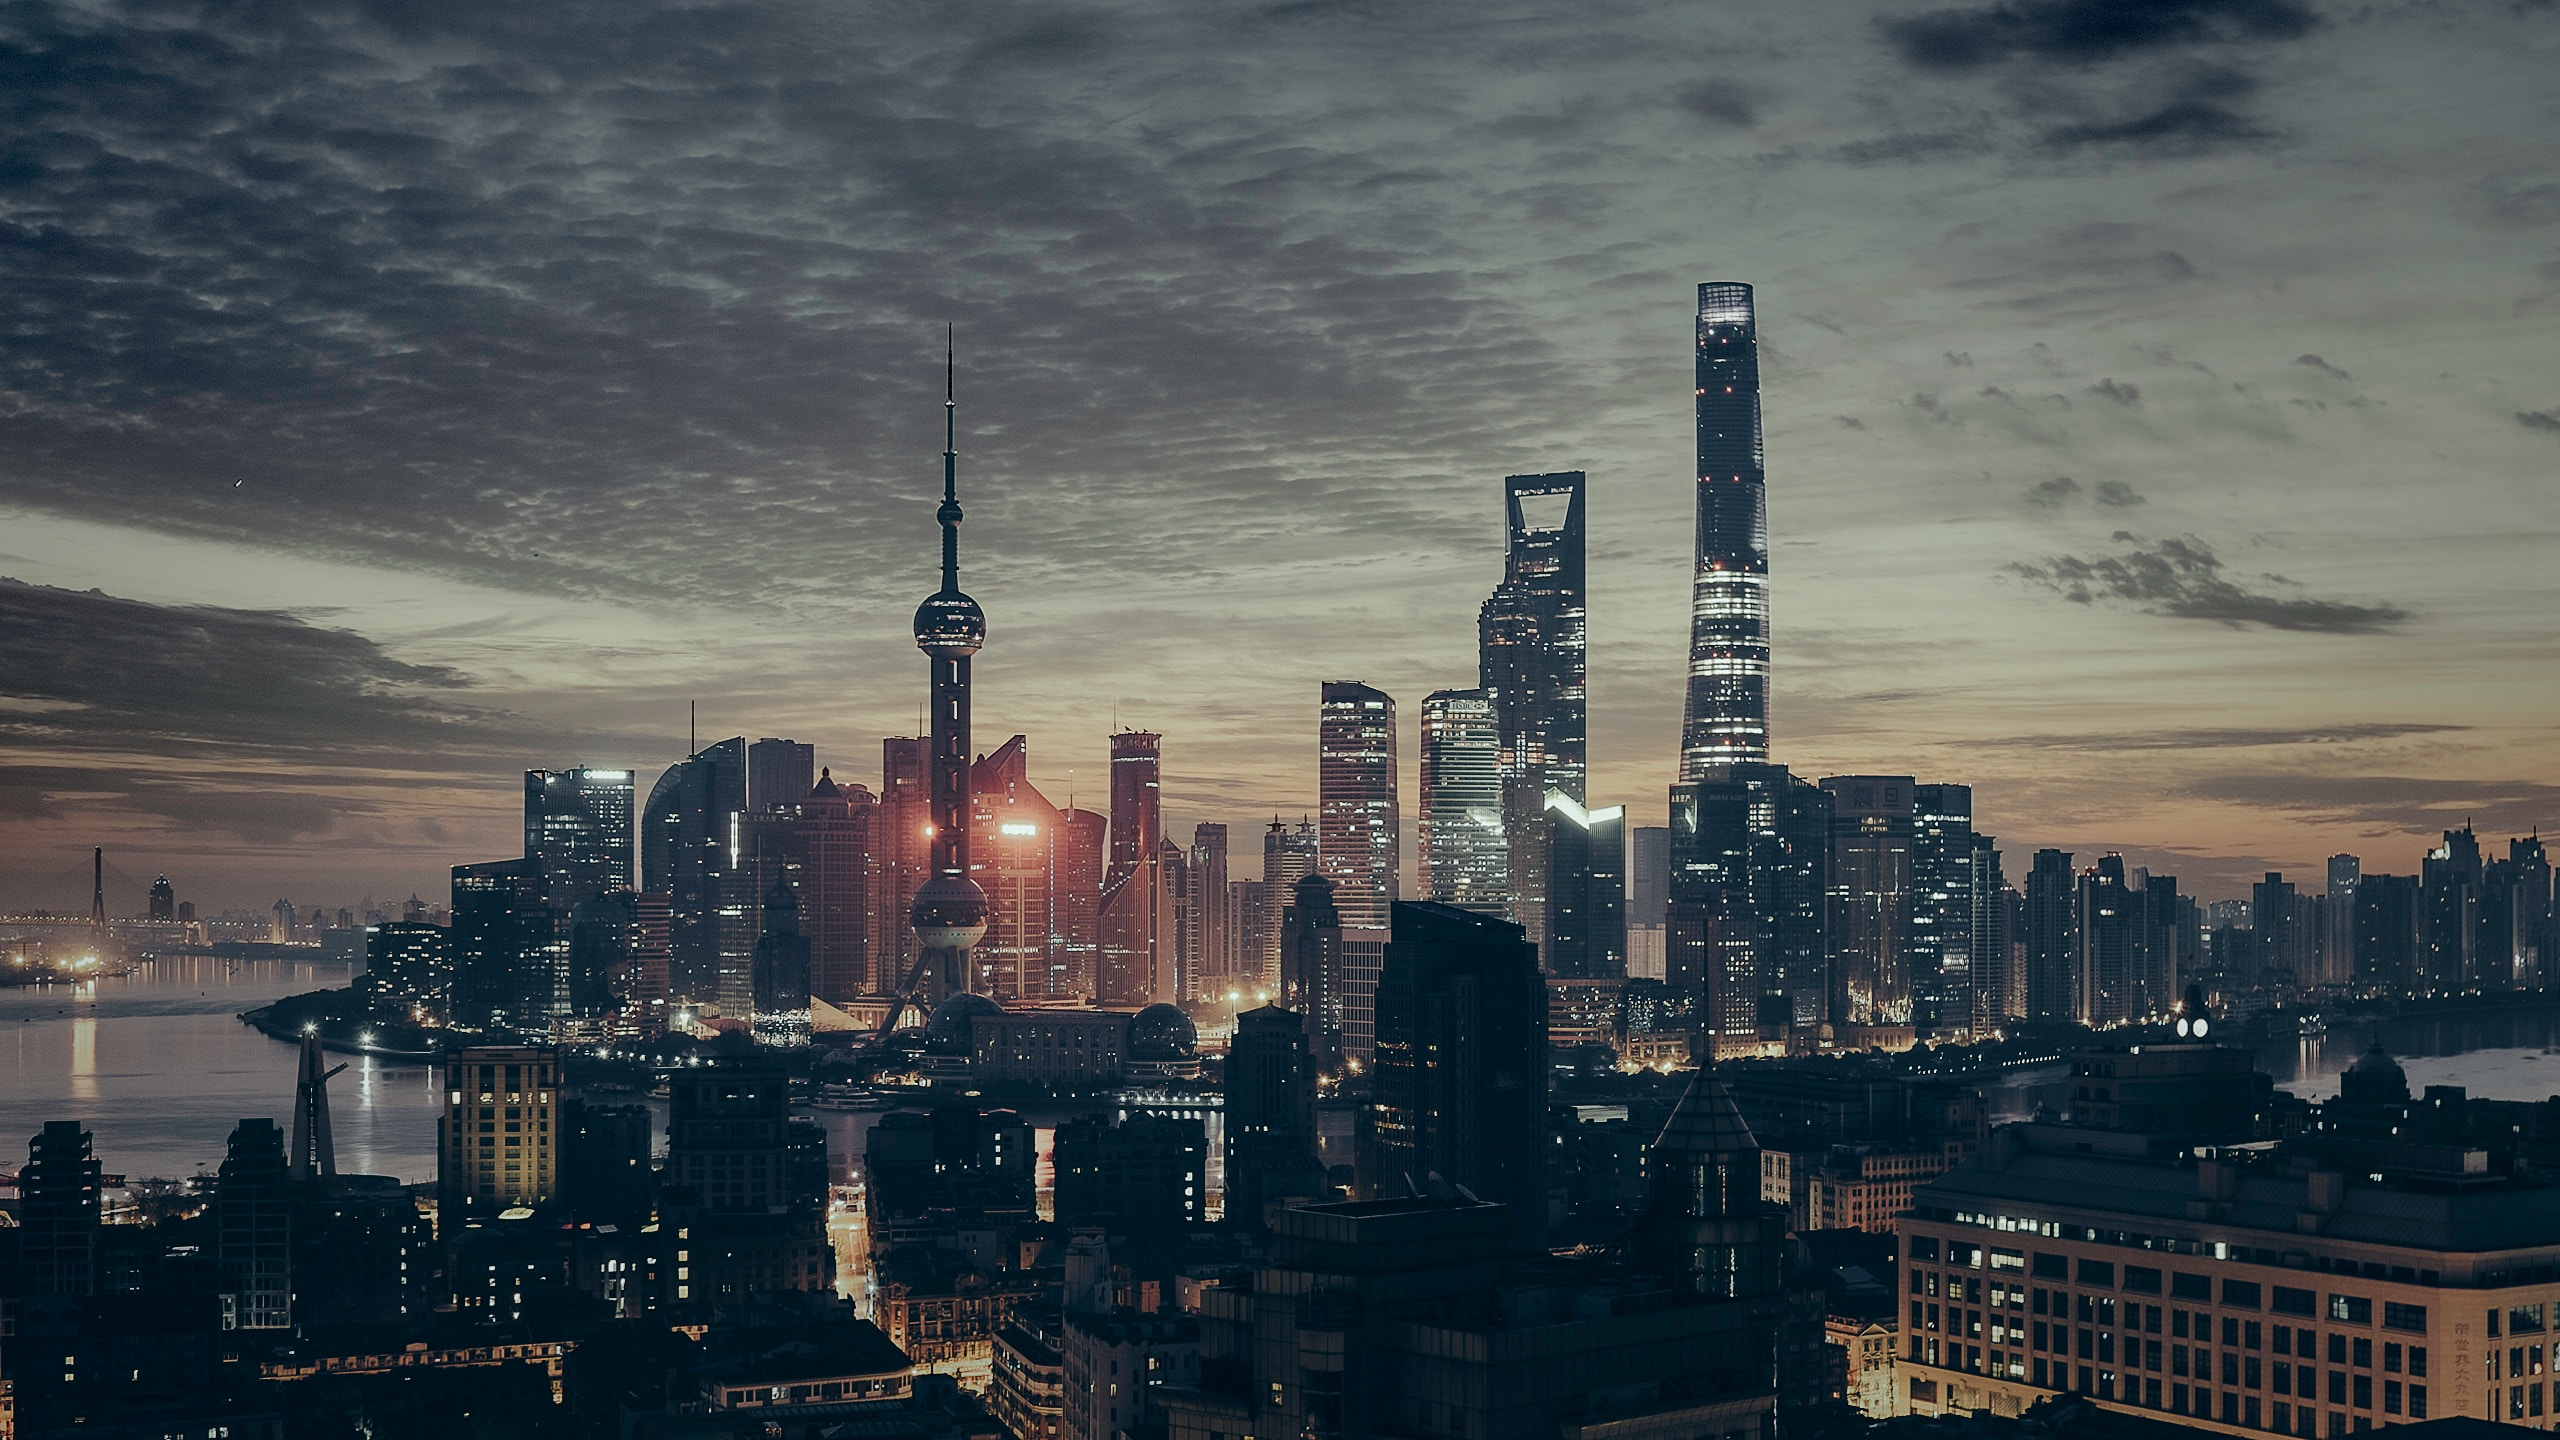
\includegraphics[scale = 0.5]{Img/china-illustration.jpg}
\end{center}
\end{figure}
\author{\Large{Marie \bsc{Chiaverini}} \Large{Baptiste  \bsc{Saclier}} \\\Large{Vadim  \bsc{Crochet}} \Large{Antoine  \bsc{Caillet}} \\\Large{Romain  \bsc{Junca}}}
\date{}
\vfill 
\end{titlepage}
\maketitle
\vspace{5.5cm}
\Large{CESI school of engineers} \hfill \Large{Tutor : Thierry \bsc{BLANC}}
\thispagestyle{empty}
\setcounter{page}{0}
\newpage

\renewcommand{\contentsname}{\Huge{Table of contents}}
\tableofcontents

\newpage
\renewcommand{\listfigurename}{\Huge{List of figures}}
\listoffigures

\newpage

\newcommand{\projectname}{ChineseTooth\xspace}
\newcommand{\modco}{MOLD \& Co.\xspace}

\section{Introduction}

This document describes all aspects of the \projectname project which the main goal is to install IT systems around the new production line in the eco-city of Taijin.
This project includes a social and ecological aspect in order to fit to the requirements of Taijin city guidelines.

In this document, we describe what are the goals, the processes, the planning and the risk of such deployment in China.

\section{Project description}

% Description précise de tout les aspects du projet
% Quel sont les objectifs ? 
% Dans quel contexte le projet évolue il ?
% Quels sont les contraintes (Environnement, Social, Temps, Législation) ?
% Quels sont les forces et les faiblesses ?

The main goal is to install a toothbrush production line in the eco-city of Taijin in China.
Our company is workig for \moldco to make this production line a reality.

Ou main guidelines in this project is to install a production line that can produce a great amount of toothbrushes within an eco-city.
This project needs to be respectful of the surrounding environnement and social aspects of the project's stakeholders.

\subsection{Specifications}

This project have to achieve the following specifications.

\paragraph{Full toothbrush production line} The production line must contains all the required machines to automate the production of toothbrushes.
Theses machines includes moulting machine, Stamping machine, Tufting machine, bristle cutter machine, bristle trimming machine and Packaging machine.

\section{Actors and Stakeholders}

% Quels sont les différents acteurs ayant un impact sur le projet ?
% Quels sont les parties prenantes et leur position dans le projet ?
% Quels sont les équipes que l'on doit mettre en place ?

\section{Project planning}

% Liste des différentes taches à éfféctuer pour atteindre les objectifs 
% Planning prévisionnel des taches
% Deadlines
% Association des équipes à chaque tache
% Quels sont les marges ? Le chemin critique ?

\section{Required resources}

% Quels sont les moyens humains nécéssaires ?
    % Equipes
    % Formations
    % Nombres d'heures
% Quels sont les moyens financiers requis ?
% Quels sont les moyens materiel requis ?

\section{Risks management}

% Quels sont les risques encourus durant le projet ?
% Quel est la sévérité, la probabilité d'apparition ?
% Quel opérations mettre en place pour les risques les plus graves ?

\section{Indicators of progression and success}

% Comment peut on quantifier l'avancement du projet ?
% Quel est l'indicateur permettant de définir qu'une tache est accomplie et valide ?

\section{Conclusion}



\end{document}

